%\documentclass[fleqn]{book}
\documentclass[11pt]{amsbook}

\usepackage[turkish]{babel}

%\usepackage{../HBSuerDemir}	% ------------------------
\usepackage{../Ceyhun}	% ------------------------
\usepackage{../amsTurkish}


\begin{document}
% ++++++++++++++++++++++++++++++++++++++
\hPage{076}
% ++++++++++++++++++++++++++++++++++++++
2.4 İkikümeli çizgeler\\
\rule{\textwidth}{1pt}\\




olarak göstereceğiz. Burada, 

\[
	d=m+n
\]

Bağlı bir Ç(d, a) çizgesinde, $\wedge_1$ ve $\wedge_2$ ortak düğümsüz iki ayrı çekirdek olsun.

\[
	\Delta=\wedge_1 \cap \wedge_2
\]

ise, 
\begin{align*} 
	d&=\lambda_1+\lambda_2 \\
	m&=\lambda_1 \\
	n&=\lambda_2
\end{align*}
	

eşitlikleri ile sağlanır ve Ç(d, a), İ(m, n) olarak gösterilen bir ikikümeli çizgedir. Şekil 2.4.3'de  bağlı ikikümeli çizgelere örnek gösterilmiştir.

%\begin{figure}[htb]
	\centering
	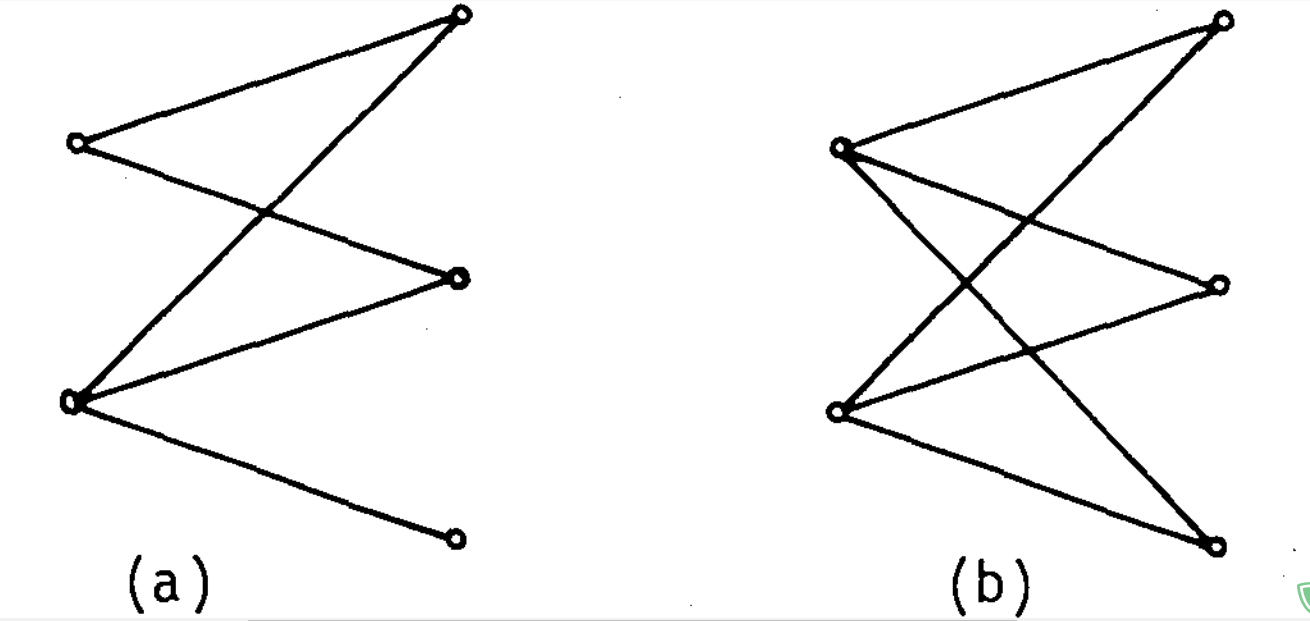
\includegraphics[width=0.45\textwidth]{images/ceyhun-076-fig01}
%	\caption{Classification of complex numbers}
%	\label{fig:classificationOfComplexNumbersA}
%\end{figure}

Şekil 2.4.3 Bağlı ikikümeli çizgeler.

\end{document}